\documentclass[11pt,a4paper]{article}
\usepackage[utf8]{inputenc}
\usepackage[german]{babel}
\usepackage[T1]{fontenc}
\usepackage{amsmath}
\usepackage{amsfonts}
\usepackage{amssymb}
\usepackage{graphicx}
\usepackage[margin=1.25cm]{geometry} % Puts the same margin on all borders of the document

% Packages

\usepackage{hyperref} % Generate hyperlinks to referenced items
\usepackage{adjustbox} % Used to change parameters in \includegraphics[scale=•]{•}
\usepackage{enumitem} % Provides several options for lists
\usepackage{verbatim} % Package to use \begin{comment}
\usepackage{pdfpages} % Used to import PDF pages
\usepackage{multirow} % Allows us to have a single cell in a table span multiple rows
\usepackage{makecell} % Allows us to format multiple lines in a single cell
\usepackage{minted} % Used to syntax highlight code
\usepackage{xcolor}  % Gives access to coloring text
\usepackage{longtable} % Allows us to create a table over multiple pages
\usepackage{float} % Improved placement of floating items
\usepackage{pdfpages} % Used to import pdf pages
\usepackage{booktabs} % Used for horizontal lines instead of \hline



% Settings

\graphicspath{{./files/}} % Sets path for files to the files folder in the same directory

\hypersetup{
    colorlinks=false, %set true if you want colored links
    linktoc=all,     %set to all if you want both sections and subsections linked
    linkcolor=blue,  %choose some color if you want links to stand out
}

%\usepackage[none]{hyphenat} If I want to disable hyphenation

\begin{titlepage}
  \title{Mathematik II für Informatik - Zusammenfassung} % document_name-type_of_document
  \author{Jonas Milkovits}
  \date{Last Edited: \today}
\end{titlepage}

\setlist{nosep} % no space between list elements

\begin{document}

\pagenumbering{gobble}
\maketitle
\pagenumbering{roman} % i, ii, iii on beginning pages, that don't have content
\tableofcontents
\clearpage
\pagenumbering{arabic} % 1,2,3 on content pages

\begin{comment}
    \noindent
    \textbf{Definitionen}
    \begin{table}[H]  
    \begin{tabularx}{\textwidth}{X m{16cm}}
        \toprule

        & \\

        \bottomrule

    \end{tabularx}
    \end{table}

    \noindent 
    \textbf{Sätze}
    \begin{table}[H]
    \begin{tabularx}{\textwidth}{X m{16cm}}
        \toprule

        & \\

        \bottomrule
    \end{tabularx}
    \end{table}

    \noindent
    \textbf{Bemerkungen}
    \begin{table}[H]
    \begin{tabularx}{\textwidth}{X m{16cm}}
        \toprule

        & \\

        \bottomrule
    \end{tabularx}
    \end{table}

    \noindent
    \textbf{Beispiele}
    \begin{table}[h]
    \begin{tabularx}{\textwidth}{X m{16cm}}
        \toprule

        & \\

        \bottomrule
    \end{tabularx}
    \end{table}
\end{comment}

\section{Analysis Teil I - Konvergenz und Stetigkeit}
\subsection{Die reellen Zahlen}
    \noindent
    \textbf{Definitionen} 
    \begin{table}[H]  
    \begin{tabularx}{\textwidth}{X m{16cm}}
        \toprule
        
        5.1.1 & Die \textbf{Menge der reellen Zahlen} ist der kleinste angeordnete Körper, 
                der $\mathbb{Z}$ enthält und das Vollständigskeitsaxiom 
                \textit{"Jede nichtleere Teilmenge, die eine obere Schranke besitzt, hat ein Suprenum."}
                erfüllt. \\
        \midrule
        5.1.3 & Eine Teilmenge $M \subseteq \mathbb{R}$ heißt:
                \begin{itemize}[topsep=-0.5cm]
                    \item[a)] nach \textbf{oben (unten) beschränkt}, wenn sie eine obere (untere) Schranke besitzt.
                    \item[b)] \textbf{beschränkt}, wenn sie nach oben und unten beschränkt ist. 
                \end{itemize} \vspace{-0cm} \\
        \midrule
        5.1.5 & Die Funktion $|\cdot|: \mathbb{R} \rightarrow \mathbb{R}$ mit \hfill \break
                \centerline{    
                    $|x| =  \begin{cases}
                    x & \text{falls x $\geq$ 0} \\
                    -x & \text{falls x < 0}
                \end{cases}$
                } \hfill \break
                heißt \textbf{Betragsfunktion} und $|x|$ heißt Betrag von $x$. \\
        \midrule
        5.1.8 & \textbf{Intervalle:} \hfill \break 
                Es seien zwei Zahlen $a,b \in \mathbb{R}$ mit $a < b$ gegeben. Dann heißen:
                \begin{itemize}[topsep=-0.5cm]
                    \item $(a,b):= \{x \in \mathbb{R}: a < x < b\}$ offenes Intervall
                    \item $[a,b]:= \{x \in \mathbb{R}: a \leq x \leq b\}$ abgeschlossenes Intervall
                    \item $(a,b]:= \{x \in \mathbb{R}: a < x \leq b\}$ halboffenes Intervall
                    \item $[a,b):= \{x \in \mathbb{R}: a \leq x < b\}$ halboffenes Intervall
                \end{itemize} \vspace{-0cm} \hfill \break
                \textbf{Halbstrahlen:}
                \begin{itemize}[topsep=-0.5cm]
                    \item $[a,\infty) := \{x \in \mathbb{R} : a \leq x\}$
                    \item $(a, \infty) := \{x \in \mathbb{R} : a < x\}$
                    \item $(-\infty, a] := \{x \in \mathbb{R}: x \leq a\}$
                    \item $(-\infty,a) := \{x \in \mathbb{R} : x < a\}$
                    \item $(-\infty,\infty):= \mathbb{R}$
                \end{itemize} \vspace{-0cm} \\
        \bottomrule
        
    \end{tabularx}
    \end{table}

    \noindent
    \textbf{Sätze}
    \begin{table}[H]
    \begin{tabularx}{\textwidth}{X m{16cm}}
        \toprule

        5.1.4 & Jede nach unten beschränkte, nichtleere Teilmenge von $\mathbb{R}$ besitzt ein Infimum. \linebreak
                (Umkehrung Vollständigkeitsaxiom) \\
        \midrule
        5.1.6 & \textbf{Rechenregeln Betragsfunktion:} \hfill \break
                Für alle $x,y \in \mathbb{R}$ gilt: 
                \begin{itemize}[topsep=-0.5cm]
                    \item[a)] $|x| \geq 0$
                    \item[b)] $|x| = |-x|$
                    \item[c)] $\pm x \leq |x|$
                    \item[d)] $|xy| = |x| \cdot |y|$
                    \item[e)] $|x| = 0$ genau dann, wenn $x = 0$
                    \item[f)] $|x+y| \leq |x| + |y|$ (Dreiecksungleichung)  
                \end{itemize} \vspace{-0cm} \\

        

        \bottomrule
    \end{tabularx}
    \end{table}

    \noindent
    \textbf{Bemerkungen}
    \begin{table}[H]
    \begin{tabularx}{\textwidth}{X m{16cm}}
        \toprule

            &   Ein Körper mit Totalordnung $\leq$ heißt \textbf{angeordneter Körper}, falls gilt:
                \begin{itemize}[topsep=-0.5cm]
                    \item $\forall a,b,c \in K: a \leq b \Rightarrow a + c \leq b + c$
                    \item $\forall a,b,c \in K: (a \leq b$ und $0 \leq c) \Rightarrow ac \leq bc$
                \end{itemize} \vspace{-0cm} \\

        \bottomrule
    \end{tabularx}
    \end{table}

    \pagebreak

\subsection{Wurzeln, Fakultäten und Binomialkoeffizienten}
    \noindent
    \textbf{Definitionen}
    \begin{table}[H]  
    \begin{tabularx}{\textwidth}{X m{16cm}}
        \toprule
        
        5.2.1 & \textbf{Ganzzahlige Potenzen:} \hfill \break
                Für jedes $x\in \mathbb{R}$ und jedes $n \in \mathbb{N^*}$ ist
                \begin{itemize}[topsep=-0.5cm]
                    \item[a)] $x^n := x \cdot x \cdot x ... \cdot x$ ($n$-mal $x$)
                    \item[b)] $x^{-n} := \frac{1}{x^n}$, falls $x\neq 0$
                    \item[c)] $x^0 := 1$  
                \end{itemize} \vspace{-0cm} \\
        \midrule
        5.2.3 & Es seien $a \in \mathbb{R_+}$ und $n \in \mathbb{N^*}$. Die \textbf{eindeutige Zahl} $x^n \in \mathbb{R_+}$ mit 
                $x^n = a$ heißt $n$-te \textbf{Wurzel} von $a$ und man schreibt $x = \sqrt[n]{a}$. Für den wichtigsten Fall $n = 2$ 
                gibt es die Konvention $\sqrt{a} := \sqrt[2]{a}$. \\
        \midrule
        5.2.5 & Aus der Eindeutigkeit der $n$-ten Wurzel (5.2.4) folgt: \hfill \break
                Für jedes $x \in \mathbb{R_+}$ und jedes $q = \frac{n}{m} \in \mathbb{Q}$ mit $n \in \mathbb{Z}$ und 
                $m \in \mathbb{N^*}$ ist die \textbf{rationale Potenz} definiert durch: \hfill \break
                \centerline{$x^q = x^{\frac{n}{m}} := (\sqrt[x]{x})^n$.} \\
        \midrule
        5.2.7 & Es sei $n \in \mathbb{N^*}$. Dann wird die Zahl $n! := 1 \cdot 2 \cdot ... \cdot n$ als $n$ \textbf{Fakultät} bezeichnet. \hfill \break
                Weiterhin definieren wir $0! := 1$. \hfill \break
                Es seien $n,k \in \mathbb{N}$ mit $k \leq n$. Dann heißt $\binom{n}{k} := \frac{n!}{k!(n-k)!}$ \textbf{Binomialkoeffizient} 
                \string"$n$ über $k$\string". \\
        \bottomrule
        
    \end{tabularx}
    \end{table}

    \noindent
    \textbf{Sätze}
    \begin{table}[H]
    \begin{tabularx}{\textwidth}{X m{16cm}}
        \toprule

        5.2.2 & \textbf{Existenz der Wurzel:} \hfill \break 
                Für jedes $a \in R_+$ und alle $n \in N^*$ gibt es genau ein $w \in R_+$ mit $x^n = a$. \\
        \midrule
        5.2.4 & Es seien $q \in \mathbb{Q}$ und $m,ü \in \mathbb{Z}$, sowie $n,r \in \mathbb{N^*}$ so, dass
                $q = \frac{m}{n} = \frac{p}{r}$. \hfill \break
                Dann gilt für jedes $x \in \mathbb{R_+}$: $(\sqrt[n]{x})^m = (\sqrt[r]{m})^p$. \\
        \midrule
        5.2.9 & Es seien $n,k \in \mathbb{N}$ mit $k \leq n$ und $a,b \in \mathbb{R}$. Dann gilt:
                \begin{itemize}[topsep=-0.5cm]
                    \item[a)] $\binom{n}{0} = \binom{n}{n} = 1$ und $\binom{n}{k} + \binom{n}{k-1} = \binom{n+1}{k}$
                    \item[b)] $a^{n+1} - b^{n+1} = (a-b) \sum^n_{k=0}a^{n-k}b^k$
                    \item[c)] $(a+b)^n = \sum^n_{k=0} \binom{n}{k} a^{n-k}b^k$ (Binomialformel)  
                \end{itemize} \vspace{-0cm} \\
        

        \bottomrule
    \end{tabularx}
    \end{table}

    \noindent
    \textbf{Bemerkungen}
    \begin{table}[H]
    \begin{tabularx}{\textwidth}{X m{16cm}}
        \toprule

        5.2.6 & \textbf{Rechenregeln für Potenzen (auch rational)} \hfill \break
                $\forall x,y \in \mathbb{R_+} \textbackslash \{0\}$ und $\forall p,q \in \mathbb{Q}$ gilt: 
                \begin{itemize}[topsep=-0.5cm]
                    \item $x^p x^q = x^{p+q}$
                    \item $x^py^p = (xy)^p$
                    \item $(x^p)^q = x^{pq}$
                    \item $\frac{x^p}{x^q} = x^{p-q}$
                    \item $\frac{x^p}{y^p} = (\frac{x}{y})^p$
                \end{itemize} \vspace{-0cm} \\
        \midrule
        5.2.8 & \textbf{Fakultät und Binomialkoeffizient} \hfill \break
                $n!$ ist die Anzahl der möglichen Reihenfolgen von $n$ unterschiedlichen Dingen. \hfill \break
                $\binom{n}{k}$ ist die Anzahl der Möglichkeiten aus $n$ unterscheidbaren Dingen genau $k$ auszuwählen. \\
        \midrule
            & Zugriff auf \textbf{Binomialkoeffizienten} für binomische Formeln durch Pascal'sches Dreieck \\
        \bottomrule
    \end{tabularx}
    \end{table}

\subsection{Konvergenz von Folgen}
\subsubsection{Der Konvergenzbegriff und wichtige Beispiele}

    \noindent
    \textbf{Definitionen}
    \begin{table}[H]  
    \begin{tabularx}{\textwidth}{X m{16cm}}
        \toprule
        
        5.3.1 & Es sei $(a_n)$ eine Folge in $\mathbb{K}$ und $a \in \mathbb{K}$. Die Folge $(a_n)$ heißt \textbf{konvergent} gegen $a$,
                falls für jedes $\epsilon > 0$ ein $n_0 \in \mathbb{N}$ exisitert mit \hfill \break
                \centerline{$|a_n-a| < \epsilon$ für alle $n \geq n_0$.}
                In diesem Fall heißt $a$ der \textbf{Grenzwert} oder Limes von $(a_n)$ und wir schreiben: \hfill \break
                \centerline{$lim_{a \rightarrow \infty} = a$ oder $a_n \rightarrow a (n \rightarrow \infty)$.} 
                Ist $(a_n)$ eine Folge $\mathbb{K}$, die gegen kein $a \in \mathbb{K}$ konvergiert, so heißt diese \textbf{divergent}. \\
        \midrule
        5.3.4 & Eine Folge $(a_n)$ in $\mathbb{K}$ heißt \textbf{beschränkt}, wenn die Menge $\{a_n: n \in \mathbb{N}\} = \{a_0,a_1,a_2,...\}$
                beschränkt in $\mathbb{K}$ ist. \hfill \break
                Ist $\mathbb{K} = \mathbb{R}$, so setzen wir weiter \hfill \break
                \centerline{$sup_{n \in \mathbb{N}}a_n := sup^{\infty}_{n=0}a_n := sup\{a_n: n \in \mathbb{N}\}$} 
                \centerline{$inf_{n \in \mathbb{N}}a_n := inf^{\infty}_{n=0}a_n := inf\{a_n: n \in \mathbb{N}\}$} \\
        \midrule
        5.3.13& \textbf{Bestimmte Divergenz:} \hfill \break
                Eine Folge $(a_n)$ in $\mathbb{R}$ \textbf{divergiert bestimmt nach $\infty (- \infty)$} und wir schreiben
                $lim_{n \rightarrow \infty} a_n = \infty (-\infty)$, wenn es für jedes $C \geq 0$ ein $n_0 \in \mathbb{N}$ gibt, so dass
                $a_n \geq C (a_n \leq -C)$ für alle $n \leq n_0$ gilt. \\


        \bottomrule
        
    \end{tabularx}
    \end{table}

    \noindent 
    \textbf{Sätze}
    \begin{table}[H]
    \begin{tabularx}{\textwidth}{X m{16cm}}
        \toprule

        5.3.5 & Jede \textbf{konvergente Folge} in $\mathbb{K}$ ist \textbf{beschränkt}. \hfill \break
                Die Umkehrung dieses Satzes ist \textbf{falsch}. Es gibt beschränkte Folgen, die nicht konvergieren. \\
        \midrule
        5.3.7 & \textbf{Grenzwertsätze} \hfill \break
                Es seien $(a_n), (b_n)$ und $(c_n)$ Folgen in $\mathbb{K}$. Dann gilt:
                \begin{itemize}
                    \item[a)] Ist $lim_{n\rightarrow \infty} a_n = a$, so gilt $lim_{n \rightarrow \infty} |a_n| = |a|$
                    \item[b)] Gilt $lim_{n \rightarrow \infty} a_n = a$ und $lim_{n \rightarrow \infty} b_n = b$ so gilt:
                        \begin{itemize}
                            \item[i)] $lim_{n \rightarrow \infty}(a_n + b_n) = a + b$
                            \item[ii)] $lim_{n \rightarrow \infty} (a_n \cdot b_n) = a \cdot b$
                            \item[iii)] $lim_{n \rightarrow \infty} (\alpha a_n) = \alpha a$ für alle $\alpha \in \mathbb{K}$
                            \item[iv)] Ist zusätzlich $b_n \neq 0$ für alle $n \in \mathbb{N}$ und $b \neq 0$, 
                                        so ist $lim_{n \rightarrow \infty} \frac{a_n}{b_n} = \frac{a}{b}$
                        \end{itemize} 
                \end{itemize}
                Ist $\mathbb{K} = \mathbb{R}$, so gilt außerdem:
                \begin{itemize}[topsep=-0.5cm]
                    \item[c)] Ist $a_n \leq b_n$ für alle $n \in \mathbb{N}$ und $lim_{n \rightarrow \infty} a_n = a$ sowie 
                                $lim_{n \rightarrow \infty} b_n = b$, so folgt $a \leq b$
                    \item[d)] Ist $a_n \leq c_n \leq b_n$ für alle $n \in \mathbb{N}$ und sind $(a_n)$ und $(b_n)$ konvergent mit
                                $lim_{n \rightarrow \infty} a_n = lim_{n \rightarrow \infty} b_n = a$, so ist auf die Folge $(c_n)$
                                konvergent und es gilt $lim_{n \rightarrow \infty} c_n = a$ \hfill \break
                                \textbf{(Sandwich-Theorem)} 
                \end{itemize} \vspace{-0cm} \\


        \bottomrule
    \end{tabularx}
    \end{table}

    \noindent
    \textbf{Bemerkungen}
    \begin{table}[H]
    \begin{tabularx}{\textwidth}{X m{16cm}}
        \toprule

            & Sei $X$ eine Menge. Eine \textbf{Folge} in $X$ ist eine Abbildung $a: \mathbb{N} \rightarrow X$. \hfill \break
                (Für $X = \mathbb{R}$ reelle Folge, $X = \mathbb{C}$ komplexe Folge) \hfill \break
                Schreibweise: $a_n$ statt $a(n)$. ($n$-tes Folgeglied) \hfill \break
                Ganze Folge: $(a_n)_{n \in \mathbb{N}}$ oder $(a_n)$ oder $(a_n)_{n>0}$ \\
        \midrule
            & Folgen haben maximal einen (eindeutiger) Grenzwert \\
        \midrule
            & Bezeichnung von Folgen, für die der Grenzwert 0 ist: \textbf{\string"Nullfolge\string"} \\
        \midrule
        5.3.7 & c) ist falsch mit $<$, nur richtig mit $\leq$ \\
        \midrule
        5.3.10& \textbf{Wichtige konvergente Folgen}
                \begin{itemize}[topsep=-0.5cm]
                    \item[a)] Ist $(a_n)$ eine konvergente Folge in $\mathbb{R}$ mit Grenzwert $a$ und gilt $a \geq 0$ für alle $n \in \mathbb{N}$
                                so ist für jedes $p \in \mathbb{N^*}$ auch $lim_{n \rightarrow \infty} \sqrt[p]{a_n} = \sqrt[p]{a}$.
                    \item[b)] Die Folge $(q^n)_{n \in \mathbb{N}}$ mit $q \in \mathbb{R}$ konvergiert genau dann, wenn $q \in (-1,1]$ ist
                                und es gilt: \hfill \break
                                $lim_{n \rightarrow \infty} q^n =   \begin{cases}
                                                                    1 & \text{falls $q = 1$} \\
                                                                    0 & \text{falls $-1 < q < 1$}
                                                                    \end{cases}$ \hfill \break
                                Ist $q \in \mathbb{C}$ mit $|q| < 1$, so gilt ebenfalls $lim_{n \rightarrow \infty} q^n = 0$.
                    \item[c)] $lim_{n \rightarrow \infty} \sqrt[n]{c} = 1$ für jedes $c \in \mathbb{R_+}$.
                    \item[d)] $lim_{n \rightarrow \infty} \sqrt[n]{n} = 1$.
                    \item[e)] $lim_{n \rightarrow \infty} (1 + \frac{1}{n})^n := e$ ($n \geq 1$). \hfill \break
                                Beachte hier: Beide $n$ gleichzeitig wachsen lassen, keine trägen oder eiligere $n$.
                \end{itemize} \vspace{-0cm} \\
        
        
        \bottomrule
    \end{tabularx}
    \end{table}

    \noindent
    \textbf{Beispiele}
    \begin{table}[H]
    \begin{tabularx}{\textwidth}{X m{16cm}}
        \toprule

        5.3.1 & Folge $(a_n) = (\frac{1}{n})_{n\geq 1} = (1, \frac{1}{2}, \frac{1}{3},...)$ \hfill \break
                Sei $\epsilon > 0$. Dann $\frac{1}{\epsilon} < n_0$ für ein $n_0 \in \mathbb{N}$ (beliebiges $n$ immer größer). \hfill \break 
                Für alle $n \geq n_0$ gilt dann: \hfill \break
                \centerline{$|a_n - a| = |a_n - 0| = |a_n| = \frac{1}{n} \leq \frac{1}{n_0} < \epsilon$}
                $\Rightarrow$ Konvergenz gegen 0 \\
        \midrule
        5.3.9 & Sei $p \in \mathbb{N^*}$ fest gewählt und $a_n = \frac{1}{n^p}$ für $n \in \mathbb{N^*}$. Dann gilt für alle
                $n \in \mathbb{N^*}$ die Ungleichung $n \leq n^p$ und damit \hfill \break
                \centerline{$0 \leq a_n = \frac{1}{n^p} \leq \frac{1}n{}$.}
                Da sowohl die Folge, die konstant Null ist, als auch die Folge $\frac{1}{n}$ gegen Null konvergiert,
                ist damit nach Satz $5.3.7(d)$ auch die Folge $(a_n)$ konvergent und ebenfalls eine Nullfolge. \\
        \midrule
        5.3.9 & Wir untersuchen \hfill \break
                \centerline{$a_n = \frac{n^2 + 2n + 3}{n^2 + 3}$, $n \in \mathbb{N}$.}
                Dazu kürzen wir durch Bruch durch die \textbf{höchste auftretende Potenz}: \hfill \break
                \centerline{$a_n = \frac{n^2 + 2n + 3}{n^2 + 3} = \frac{1 + \frac{2}{n} + \frac{3}{n^2}}{1 + \frac{3}{n^2}} \rightarrow 
                \frac{1+0+0}{1+0} = 1$ $(n \rightarrow \infty)$.} 
                Dieses Verfahren ist bei allen "Polynom in $n$ geteilt durch Polynom in $n$" gut anwendbar. \\
        \midrule
        5.3.12& $a_n := \sqrt{n + 1} - \sqrt{n}$, $n \in \mathbb{N}$ (Differenz von zwei divergenten Folgen) \hfill \break
                Trick: Erweiterung mit der Summe von Wurzeln bei Differenzen von Wurzeln \hfill \break
                \centerline{$\sqrt{n + 1} - \sqrt{n} = \frac{\sqrt{n + 1} - \sqrt{n} \sqrt{n + 1} + \sqrt{n}}{\sqrt{n + 1} + \sqrt{n}} 
                = \frac{(n+1)-n}{\sqrt{n + 1} + \sqrt{n}} = \frac{1}{\sqrt{n + 1} + \sqrt{n}} \leq \frac{1}{2\sqrt{n}} = 
                \frac{1}{2}\sqrt{\frac{1}{n}}$ }
                Sandwich: $lim_{n \rightarrow \infty}(\sqrt{n + 1} - \sqrt{n}) = 0$. \\
        \midrule
        5.3.12& \textbf{Geometrische Summenformel:} \hfill \break
                \centerline{$a_n := \sum^n_{k=0} q^k = 1 + q + q^2 + ... + q^n$, $n \in \mathbb{N}$}
                $lim_{n \rightarrow \infty} a_n = \frac{1}{1-q}$, $|q| < 1$. \\

        \bottomrule
    \end{tabularx}
    \end{table}


\subsubsection{Konvergenzkriterien}

    \noindent
    \textbf{Definitionen}
    \begin{table}[H]  
    \begin{tabularx}{\textwidth}{X m{16cm}}
        \toprule
        
        5.3.14& Eine reelle Folge $(a_n)$ heißt:
                \begin{itemize}[topsep=-0.5cm]
                    \item[a)] \textbf{monoton wachsend}, wenn $a_{n+1} \geq a_n$ für alle $n \in \mathbb{N}$ gilt.
                    \item[b)] \textbf{monoton fallend}, wenn $a_{n+1} \leq a_n$ für alle $n \in \mathbb{N}$ gilt.
                    \item[c)] \textbf{monoton}, wenn sie monoton wachsend oder monoton fallend ist. 
                \end{itemize} \vspace{-0cm} \\
        \midrule
        5.3.18& Folge $(a_n)$ in $\mathbb{K}$ heißt \textbf{Cauchy-Folge}, wenn für jedes $\epsilon > 0$ ein Index
                $n_0 \in \mathbb{N}$ existiert, so dass\hfill \break
                \centerline{$|a_n - a_m| < \epsilon$, für alle $n,m \geq n_0$} \\

        \bottomrule
        
    \end{tabularx}
    \end{table}

    \noindent 
    \textbf{Sätze}
    \begin{table}[H]
    \begin{tabularx}{\textwidth}{X m{16cm}}
        \toprule

        5.3.15& \textbf{Monotonie Kriterium} \hfill \break
                Ist die reelle Folge $(a_n)$ nach oben (nach unten) beschränkt und monoton wachsend (fallend), so ist $(a_n)$ \textbf{konvergent}
                und es gilt: \hfill \break
                \centerline{$lim_{n \rightarrow \infty} a_n = sup_{n \in \mathbb{N}}a_n$ (bzw. $lim_{n \rightarrow \infty} a_n = inf_{n \in \mathbb{N}}a_n$) } \\
        \midrule
        5.3.19& Jede konvergente Folge in $\mathbb{K}$ ist eine \textbf{Cauchy-Folge}. \\
        \midrule
        5.3.20& \textbf{Cauchy-Kriterium} \hfill \break
                Eine Folge in $\mathbb{K}$ konvergiert genau dann, wenn sie eine Cauchy-Folge ist. \\
        \bottomrule
    \end{tabularx}
    \end{table}

    \noindent
    \textbf{Bemerkungen}
    \begin{table}[H]
    \begin{tabularx}{\textwidth}{X m{16cm}}
        \toprule

            & Monotonieverhalten, deswegen hier nur in $\mathbb{R}$ und nicht in $\mathbb{C}$ (keine Ordnung) \\
            \midrule
            & Beide hier gesehenen Konvergenzkriterien funktionieren ohne vorherige Behauptung über den Grenzwert \\  
            
        \bottomrule
    \end{tabularx}
    \end{table}

    \noindent
    \textbf{Beispiele}
    \begin{table}[h]
    \begin{tabularx}{\textwidth}{X m{16cm}}
        \toprule

        5.3.16& Betrachtung einer rekursiv defininierten Folge \hfill \break
                \centerline{$a_0 := \sqrt[3]{6}$ und $a_{n+1} = \sqrt[3]{6 + a_n}, n \in \mathbb{N}$} 
                Damit folgt: $a_1 = \sqrt[3]{6+\sqrt[3]{6}}$, $a_2 = \sqrt[3]{6+\sqrt[3]{6+\sqrt[3]{6}}}$ \hfill \break
                Solche Folgen entstehen oft bei iterativen Näherungsverfahren. \hfill \break
                Behauptung: $(a_n)$ nach oben beschränkt und monoton wachsend $\Rightarrow$ Konvergenz \hfill \break
                Beweis: Induktion  \\

        \bottomrule
    \end{tabularx}
    \end{table}

\subsubsection{Teilfolgen und Häufungswerte}
    \noindent
    \textbf{Definitionen}
    \begin{table}[H]  
    \begin{tabularx}{\textwidth}{X m{16cm}}
        \toprule
        
        5.3.22& Es sei $(a_n)$ eine Folge in $\mathbb{K}$. Ein $a \in \mathbb{K}$ heißt Häufungswert der Folge, falls für jedes
                $\epsilon > 0$ die Menge $\{n \in \mathbb{N}: |a_n -a| < \epsilon\}$ unendlich viele Elemente hat. \\
        \midrule
        5.3.23& Es sei $(a_n)$ eine Folge in $\mathbb{K}$. Ist $\{n_1,n_2,n_3,...\} \subseteq \mathbb{N}$ eine unendliche Menge 
                von Indizes mit $n_1 < n_2 < n_3 ...$, so heißt die Folge $(a_{n_k}))_{k \in \mathbb{N}}$ eine Teilfolge von $(a_n)$. \\

        \bottomrule
        
    \end{tabularx}
    \end{table}

    \noindent 
    \textbf{Sätze}
    \begin{table}[H]
    \begin{tabularx}{\textwidth}{X m{16cm}}
        \toprule

        5.3.24& Es sei $(a_n)$ eine Folge in $\mathbb{K}$. Dann gilt \hfill \break
                \begin{itemize}
                    \item[a)] Ein $\alpha \in \mathbb{K}$ ist genau dann ein Häufungswert von $(a_n)$, wenn eine Teilfolge $(a_{n_k})$ von
                                $(a_n)$ existiert, die gegen $\alpha$ konvergiert.
                    \item[b)] Ist $(a_n)$ konvergenz mit Grenzwert $\alpha$, so konvergiert auch jede Teilfolge von $(a_n)$ gegen a.
                    \item[c)] Ist $(a_n)$ konvergenz, so hat $(a_n)$ genau einen Häufungswert, nämlich den Grenzwert 
                                $lim_{n \rightarrow \infty} a_n$.
                \end{itemize} \\

        \bottomrule
    \end{tabularx}
    \end{table}

    \noindent
    \textbf{Bemerkungen}
    \begin{table}[H]
    \begin{tabularx}{\textwidth}{X m{16cm}}
        \toprule

        & Jeder Grenzwert ist auch Häufungswert. \\
        \midrule
        & Häufungswert von $((-1)^n)_{n \in \mathbb{N}}$: 1, -1 (aber keine Grenzwerte) \\
        \midrule
        & Häfungswert von $(i^n)$: 1, i, -1, -i \\
        \midrule
        & Keine Teilfolgen: \hfill \break
            $(a_0, a_0, a_2, a_2,..)$ (keine doppelten Elemente) \hfill \break
            $(a_2, a_3, a_0,..)$ (nicht umsortieren) \\


        \bottomrule
    \end{tabularx}
    \end{table}

\subsection{Asymptotik}
    \noindent
    \textbf{Definitionen}
    \begin{table}[H]  
    \begin{tabularx}{\textwidth}{X m{16cm}}
        \toprule
        
        5.4.1 & \begin{itemize}
                    \item[a)] Wir bezeichnen mit $F_+ := \{(a_n)$ Folge in $\mathbb{R}: a_n > 0$ für alle $n \in \mathbb{N} \}$
                    \item[b)] Es sei $(b_n) \in \mathbb{F_+}$. Dann definieren wir die Landau-Symbole durch \hfill \break
                        \begin{itemize}
                            \item $O(b_n) := \{(a_n) \in \mathbb{F_+} : \frac{a_n}{b_n}_{n \in \mathbb{N}}\}$ ($b_n$ größer gleich $a_n$)
                            \item $o(b_n) := \{(a_n) \in \mathbb{F_+}: lim_{n \rightarrow \infty} \frac{a_n}{b_n} = 0\}$ ($b_n$ echt größer als $a_n$)
                        \end{itemize}   
                \end{itemize} \\

        \bottomrule
        
    \end{tabularx}
    \end{table}

    \noindent 
    \textbf{Sätze}
    \begin{table}[H]
    \begin{tabularx}{\textwidth}{X m{16cm}}
        \toprule

        5.4.5 & Es seien $(a_n), (b_n), (c_n), (d_n) \in \mathbb{F_+}$ und $\alpha, \beta \in \mathbb{R_+}$. Dann gilt: \hfill \break
                \begin{itemize}
                    \item[a)] Sind $a_n, b_n \in O(c_n)$, so ist auch $\alpha a_n + \beta b_n \in O(c_n)$
                    \item[b)] Gilt $a_n \in O(b_n)$ und $c_n \in O(d_n)$, so ist $a_n c_n \in O(b_n d_n)$
                    \item[c)] Aus $a_n \in O(b_n)$ und $b_n \in O(c_n)$ folgt $a_n \in O(c_n)$
                    \item[d)] $a_n \in O(b_n)$ genau dann, wenn $\frac{1}{b_n} \in O(\frac{1}{a_n})$
                    \item[e)] Diese Aussagen gelten auch alle mit Klein-O anstatt Gro\ss-O 
                \end{itemize} \\

        \bottomrule
    \end{tabularx}
    \end{table}

    \noindent
    \textbf{Bemerkungen}
    \begin{table}[H]
    \begin{tabularx}{\textwidth}{X m{16cm}}
        \toprule

        5.4.2 & \begin{itemize}
                    \item[a)] $=$-Zeichen wird hier nicht bekannten mathematischen Sinne verwendet
                    \item[] $\Rightarrow$ Kompromiss Notation $a_n \in O(b_n)$ 
                    \item[b)] Es gilt immer $o(b_n) \subseteq O(b_n)$. 
                    \item[c)] $(\frac{a_n}{b_n})_{n \in \mathbb{N}}$ konvergent $\Rightarrow$ $a_n \in O(b_n)$
                    \item[d)] $a_n \in O(b_n)$: Folge $a_n$ wächst höchstens so schnell wie ein Vielfaches von $b_n$  
                \end{itemize} \\
        \midrule
            & Exponentielle Algorithmen sind viel schlechter als polynomiale. \\
        \midrule
            & 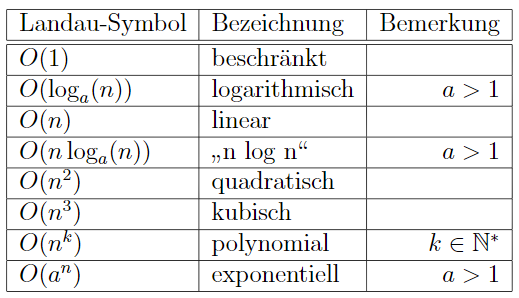
\includegraphics[width=7cm]{landau.PNG} \\

        \bottomrule
    \end{tabularx}
    \end{table}

\subsection{Reihen}
    \noindent
    \textbf{Definitionen}
    \begin{table}[H]  
    \begin{tabularx}{\textwidth}{X m{16cm}}
        \toprule

        5.5.1 & Es sei $(a_n)$ eine Folge in $\mathbb{K}$. Dann heißt \hfill \break
                \centerline{$\sum^{\infty}_{n=0} a_n = a_o + a_1 + a_2 + ... $}
                die \textbf{Reihe} über $(a_n)$. \hfill \break
                Für jedes $k \in \mathbb{N}$ heißt dann $s_k = \sum^{k}_{n=0} a_n$ die $k$-te Teilsumme oder \textbf{Partialsumme} der Reihe. \hfill \break
                Ist die Folge $(s_k)_{k \in \mathbb{N}}$ konvergent, so nennen wir die Reihe \textbf{konvergent} mit dem Reihenwert: \hfill \break
                \centerline{$\sum^{\infty}_{n=0} a_n := lim_{k \rightarrow \infty} s_k = lim_{k \rightarrow \infty} \sum^{k}_{n=0} a_n$}.
                Ist $(s_k)$ divergent, so nennen wir auch die Reihe divergent.  \\

        \bottomrule

    \end{tabularx}
    \end{table}

    \noindent 
    \textbf{Sätze}
    \begin{table}[H]
    \begin{tabularx}{\textwidth}{X m{16cm}}
        \toprule

        5.5.3 & Seien $\sum^{\infty}_{n=0} a_n$ und $\sum^{\infty}_{n=0} b_n$ zwei konvergente Reihen in $\mathbb{K}$ und 
                $\alpha, \beta \in \mathbb{K}$. Dann ist auch $\sum^{\infty}_{n=0} (\alpha a_n + \beta b_n)$ konvergent und es gilt \hfill \break
                \centerline{$\sum^{\infty}_{n=0} (\alpha a_n + \beta b_n) = \alpha \sum^{\infty}_{n=0} a_n + \beta \sum^{\infty}_{n=0} b_n$}  \\
        \midrule
        5.5.4 & Es gilt $\sum^{\infty}_{n=0} \frac{1}{n!} = e$. \\
        \midrule
        5.5.5 & Ist $\sum^{\infty}_{n=0} a_n$ eine konvergente Reihe in $\mathbb{K}$, so ist $(a_n)$ eine \textbf{Nullfolge} in $\mathbb{K}$. \\
        \midrule
        5.5.6 & Es sei $(a_n)$ eine Folge in $\mathbb{K}$ und $s_k := \sum^{k}_{n=0} a_n$, $k \in \mathbb{N}$ Dann gilt:
                \begin{itemize}
                    \item[a)] \textbf{Monotonie Kriterium} \hfill \break
                                Ist $a_n \geq 0$ für alle $n \in \mathbb{N}$ und $(s_k)_{k \in \mathbb{N}}$ nach oben beschränkt, so
                                ist $\sum^{\infty}_{n=0} a_n$ konvergent.
                    \item[b)] \textbf{Cauchy-Kriterium} \hfill \break
                                Die Reihe $\sum^{\infty}_{n=0} a_n$ ist genau dann konvergent, wenn für jedes $\epsilon > 0$ ein $n_o \in \mathbb{N}$
                                existiert mit \hfill \break
                                \centerline{$|\sum^{k}_{n=l+1} a_n| < \epsilon$ für alle $k, l \in \mathbb{N}$ mit $k > l \geq n_0$.}
                \end{itemize} \\
        \midrule
        5.5.7 & \textbf{Leibniz-Kriterium} \hfill \break
                Es sei $(a_n)$ eine monoton fallende Folge in $\mathbb{R}$ mit $lim_{n \rightarrow \infty} a_n = 0$. Dann ist die 
                Reihe $\sum^{\infty}_{n=0} (-1)^n a_n$ konvergent. \\

        \bottomrule
    \end{tabularx}
    \end{table}

    \noindent
    \textbf{Bemerkungen}
    \begin{table}[H]
    \begin{tabularx}{\textwidth}{X m{16cm}}
        \toprule

        5.5.5 & Gilt nicht umgekehrt. Nullfolge ist eine Voraussetzung für eine konvergente Reihe, aber keine Garantie. \\

        \bottomrule
    \end{tabularx}
    \end{table}

    \noindent
    \textbf{Beispiele}
    \begin{table}[h]
    \begin{tabularx}{\textwidth}{X m{16cm}}
        \toprule

              & \textbf{Reihen:}
                \begin{itemize}
                    \item $\sum^{\infty}_{n=0} q^n = \frac{1}{1-q}, |q| < 1$ \textit{(Geometrische Reihe)}
                    \item $\sum^{\infty}_{n=1} \frac{1}{n(n+1)} = 1$
                    \item $\sum^{\infty}_{n=1} \frac{1}{n} = divergent$ \textit{(Harmonische Reihe)}
                    \item $\sum^{\infty}_{n=0} \frac{1}{n!} = e$
                    \item $\sum^{\infty}_{n=0} (-1)^n \frac{1}{n+1} = ln(2)$ \textit{(alternierende harmonische Reihe)} (Leibniz-Kriterium)
                    \item $\sum^{\infty}_{n=1} \frac{1}{n^{\alpha}}:$ konvergent, wenn $\alpha > 1$, sonst divergent
                \end{itemize} \\

        \bottomrule
    \end{tabularx}
    \end{table}

\subsubsection{Absolute Konvergenz}
    \noindent
    \textbf{Definitionen}
    \begin{table}[H]  
    \begin{tabularx}{\textwidth}{X m{16cm}}
        \toprule

        5.5.9 & Eine Reihe $\sum^{\infty}_{n=0} a_n$ in $\mathbb{K}$ heißt \textbf{absolut konvergent}, wenn die Reihe
                $\sum^{\infty}_{n=0} |a_n|$ in $\mathbb{K}$ konvergiert. (Summanden werden schnell genug klein, vorzeichenunabhängig)\\

        \bottomrule

    \end{tabularx}
    \end{table}

    \noindent 
    \textbf{Sätze}
    \begin{table}[H]
    \begin{tabularx}{\textwidth}{X m{16cm}}
        \toprule

        5.5.10& Jede absolut konvergente Reihe $\sum^{\infty}_{n=0} a_n$ in $\mathbb{K}$ ist auch konvergent in $\mathbb{K}$ und es
                gilt die verallgemeinerte Dreiecksungleichung \hfill \break
                \centerline{$|\sum^{\infty}_{n=0}a_n| \leq \sum^{\infty}_{n=0} |a_n|$} \\
        \midrule
        5.5.12& Es seien $(a_n)$ und $(b_n)$ reelle Folgen und $n_o \in \mathbb{N}$.
                \begin{itemize}
                    \item \textbf{Majorantenkriterium} \hfill \break 
                            Ist $|a_n| \leq b_n$ für alle $n \geq n_o$ und konvergiert die Reihe $\sum^{\infty}_{n=0}b_n$, so ist
                            $\sum^{\infty}_{n=0} a_n$ absolut konvergent.
                    \item \textbf{Minorantenkriterium} \hfill \break
                            Ist $a_n \geq b_n \geq 0$ für alle $n \geq n_0$ und divergiert die Reihe $\sum^{\infty}_{n=0}b_n$, so 
                            divergiert auch die Reihe $\sum^{\infty}_{n=0}a_n$. 
                \end{itemize} \\
        \midrule
        5.5.16& Es sei $\sum^{\infty}_{n=0}a_n$ eine Reihe in $\mathbb{K}$.
                \begin{itemize}
                    \item[a)] \textbf{Wurzelkriterium} \hfill \break
                            Existiert der Grenzwert $lim_{n \rightarrow \infty} \sqrt[n]{|a_n|}$, so ist die Reihe
                            \begin{itemize}
                                \item absolut konvergent, wenn $lim_{n \rightarrow \infty} \sqrt[n]{|a_n|} < 1$ ist
                                \item divergent, wenn $lim_{n \rightarrow \infty} \sqrt[n]{|a_n|} > 1$ ist
                            \end{itemize}
                    \item[b)] \textbf{Quotientenkriterium} \hfill \break
                            Ist $a_n \neq 0$ für alle $n \in \mathbb{N}$ und existiert der Grenzwert 
                            $lim_{n \rightarrow \infty} |\frac{a_{n+1}}{a_n}|$, so ist die Reihe
                            \begin{itemize}
                                \item absolut konvergent, wenn $lim_{n \rightarrow \infty} |\frac{a_{n+1}}{a_n}| < 1$ ist
                                \item divergent, wenn $lim_{n \rightarrow \infty} |\frac{a_{n+1}}{a_n}| > 1$ ist
                            \end{itemize}
                \end{itemize} \\

        \bottomrule
    \end{tabularx}
    \end{table}

    \noindent
    \textbf{Bemerkungen}
    \begin{table}[H]
    \begin{tabularx}{\textwidth}{X m{16cm}}
        \toprule

        5.5.10& Gilt nicht umgekehrt (alternierende harmonische Reihe)  \\
        \midrule
        5.5.10& Absolute Konvergenz: Reihenwert ist unabhängig von der Summationsreihenfolge \\
        \midrule
        5.5.12& Die Vergleichsfolge heißt jeweils konverente Majorante bzw. divergente Minorante. \\
        \midrule
        5.5.16& Liefert Wurzel-/Quotientenkriterium genau Eins, kann man daraus keine Aussage ableiten \\

        \bottomrule
    \end{tabularx}
    \end{table}

\subsubsection{Das Cauchy-Produkt}
\noindent
\textbf{Definitionen}
\begin{table}[H]  
\begin{tabularx}{\textwidth}{X m{16cm}}
    \toprule

    5.5.21& Für alle $z \in \mathbb{C}$ ist $e^z:= E(z) = \sum\limits^{\infty}_{n=0} \frac{z^n}{n!}$. \\

    \bottomrule

\end{tabularx}
\end{table}

\noindent 
\textbf{Sätze}
\begin{table}[H]
\begin{tabularx}{\textwidth}{X m{16cm}}
    \toprule

    5.5.19& Es seien $\sum^{\infty}_{n=0} a_n$ und $\sum^{\infty}_{n=0} b_n$ zwei \textbf{absolut konvergente Folgen} in $\mathbb{K}$.
            Dann konvergiert auch die Reihe $\sum^{\infty}_{n=0} \sum^{n}_{k=0} a_k b_{n-k}$ \textbf{absolut} und es gilt für
            die Reihenwerte: \hfill \break
            \centerline{$\sum\limits^{\infty}_{n=0} \sum\limits^{n}_{k=0} a_k b_{n-k} = (\sum\limits^{\infty}_{n=0} a_n) (\sum\limits^{\infty}_{n=0} b_n)$} 
            Die Reihe $\sum\limits^{\infty}_{n=0} \sum\limits^{n}_{k=0} a_k b_{n-k}$ heißt \textbf{Cauchy-Produkt} der beiden Reihen. \\
    \midrule
    5.5.20& Für alle $z,w \in \mathbb{C}$ gilt $E(z+w) = E(z)E(w)$. \\

    \bottomrule
\end{tabularx}
\end{table}

\subsection{Konvergenz in normierten Räumen}

\noindent
\textbf{Definitionen}
\begin{table}[H]  
\begin{tabularx}{\textwidth}{X m{16cm}}
    \toprule

    5.6.1 & \begin{itemize}
                \item[a)] Eine Folge $(a_n)_{n \in \mathbb{N}}$ in $V$ heißt \textbf{konvergent} gegen ein $a \in V$, wenn
                            für jedes $\epsilon > 0$ ein $n_0 \in \mathbb{N}$ existiert, so dass \hfill \break
                            \centerline{$||a_n - a||_V < \epsilon$ für alle $n \geq n_0$}
                            Die Folge heißt \textbf{divergent,} wenn sie nicht konvergent ist.
                \item[b)] Eine Folge heißt \textbf{Cauchy-Folge}, wenn es für jedes $\epsilon > 0$ ein $n_0 \in \mathbb{N}$ gibt
                            mit \hfill \break
                            \centerline{$||a_n - a_m||_V < \epsilon$ für alle $n,m \geq n_0$}
                \item[c)] Eine Reihe $\sum^{\infty}_{n=0} a_n$ in $V$ heißt \textbf{konvergent} mit Reihenwert $s \in V$, wenn die
                            Folge der Partialsummen $s_k := \sum^{\infty}_{n=0} a_n$, $k \in \mathbb{N}$, in $V$ gegen $s$ konvergiert. \hfill \break
                            Konvergiert die Reihe $\sum^{\infty}_{n=0} ||a_n||_V$ in $\mathbb{R}$ so heißt die Reihe
                            $\sum^{\infty}_{n=0}a_n$ \textbf{absolut konvergent}. \hfill \break
                            Ist die Reihe nicht konvergent, so nennt man sie \textbf{divergent}.
            \end{itemize} \\
    \midrule
    5.6.2 & Eine Menge $M \subseteq V$ hei\ss t beschränkt, falls es ein $ \geq 0$ gibt, so dass $||x||_V \leq C$ für alle 
            $x \in \mathbb{M}$ gilt. \\
    \midrule
    5.6.8 & \begin{itemize}
                \item[a)] Es seien $x_0 \in \mathbb{V}$ und $r \in (0, \infty)$. Dann heißt die Menge \hfill \break
                            $B_r(x_0) := \{x \in V: ||x-x_o||_V < r\} $ \textbf{(offene) Kugel} um $x_0$ (Mittelpunkt) mit Radius $r$.
                \item[b)] Eine Menge $M \subseteq V$ heißt \textbf{offen}, falls es für jeden Punkt $x_0 \in M$ einen Radius
                            $r > 0$ gibt, so dass $B_r(x_0) \subseteq M$ gilt.
                \item[c)] Eine Menge $M \subseteq V$ heißt \textbf{abgeschlossen}, wenn die Menge $M^c = V \ M$ offen ist.
                \item[d)] Es sei $M \subseteq V$. Ein Punkt $x_0 \in M$ heißt \textbf{innerer Punkt} von $M$, falls es ein
                            $r > 0$ gibt, so dass $B_r(x_0) \subseteq M$ ist. \hfill \break 
                            Man nennt $M^o := \{x \in M: x$ innerer Punkt von $M$\} das \textbf{Innere von $M$}.    
                              
            \end{itemize} \\
    \midrule
    5.6.13& Ist $V$ ein endlichdimensionaler normierter $\mathbb{R}$-Vektorraum, so hei\ss t eine Teilmenge $M \subseteq V$
            \textbf{kompakt}, wenn sie abgeschlossen und beschränkt ist. \\
    \midrule
    5.6.15& Es sei $(a_n)$ eine Folge in $(V, ||\cdot||_V)$.
            \begin{itemize}
                \item[a)] Ein $a \in V$ hei\ss t \textbf{Häufungswert} von $(a_n)$m falls für jedes $\epsilon > 0$ die Menge \hfill \break
                            \centerline{\{$n \in \mathbb{N} : ||a_n - a||_V < \epsilon\} = \{n \in \mathbb{N}: a_n \in B_{\epsilon}(a)\}$}
                            unendlich viele Elemente hat.
                \item[b)] Ist $\{n_1,n_2,n_3,\dots\}$ eine unendliche Teilmenge von $\mathbb{N}$ mit $n_1 < n_2 < n_3 < \dots$, so
                            hei\ss t $(a_{n_k})_{k \in \mathbb{N}}$ eine \textbf{Teilfolge} von $(a_n)$. 
            \end{itemize} \\
    \midrule
    5.6.19& Ein normierter $\mathbb{R}$-Vektorraum $(V, ||\cdot||_V)$ heißt \textbf{vollständig}, wenn jede Cauchy-Folge in $V$ konvergiert.
            Ein vollständiger normierter $\mathbb{R}$-Vektorraum wird auch \textbf{Banachraum} genannt. \hfill \break
            Wird die Norm $||\cdot||_V$ außerdem durch eine Skalarprodukt auf $V$ induziert, so nennt man $V$ \textbf{Hilbertraum}. \\


    \bottomrule

\end{tabularx}
\end{table}

\noindent 
\textbf{Sätze}
\begin{table}[H]
\begin{tabularx}{\textwidth}{X m{16cm}}
    \toprule

    5.6.5 & Es sei $(a_n)_{n \in \mathbb{N}} = ((a_{n,1}, a_{n,2}, \dots, a_{n,d})^T)_{n \in \mathbb{N}}$ eine Folge in $\mathbb{R^d}$
            mit der 2-Norm. Dann ist $(a_n)$ in $\mathbb{R^d}$ genau dann \textbf{konvergent}, wenn für jedes $j \in \{1,2,\dots,d\}$ die
            Koordinatenfolge $(a_{n,j})_{n \in \mathbb{N}}$ in $\mathbb{R}$ \textbf{konvergent} ist. In diesem Fall ist \hfill \break
            \centerline{$lim_{n \rightarrow \infty}\begin{pmatrix}a_{n,1}\\a_{n,2}\\\dots \\ a_{n,d}\end{pmatrix} =
                \begin{pmatrix} lim_{n \rightarrow \infty} a_{n,1} \\ lim_{n \rightarrow \infty} a_{n,2} \\ \dots \\
                lim_{n \rightarrow \infty} a_{n,d} \end{pmatrix}$}.
            Falls eine Komponente im Vektor divergiert, divergiert die ganze Folge. \\
    \midrule
    5.6.11& Eine Teilmenge $M$ von $V$ ist genau dann \textbf{abgeschlossen}, wenn für jede Folge in $M$, die in $V$ konvergiert,
            der Grenzwert ein Element aus $M$ ist. \\
    \midrule
    5.6.17& \textbf{Satz von Bolzano-Weierstra\ss} \hfill \break
            Sei $(V, ||\cdot||_V)$ ein endlichdimensionaler normierter Raum und $M \subseteq V$ kompakt. Dann besitzt jede Folge in $M$
            eine \textbf{konvergente Teilfolge mit Grenzwert in $M$}. \\
    \midrule
    5.6.22& \textbf{Banach'scher Fixpunktsatz} \hfill \break
            Es sei $(V, ||\cdot||_V)$ ein Banachraum $M \subseteq V$ abgeschlossen und $f: M \rightarrow M$ eine Funktion.
            Weiter existiere ein $q \in (0,1)$, so dass \hfill \break
            \centerline{$||f(x) - f(y)||_V \leq q ||x-y||_V$, für alle $x,y \in M$}
            gilt. Dann gelten die folgenden Aussagen:
            \begin{itemize}
                \item[a)] Es gibt genau ein $v \in M$ mit $f(v) = v$. (d.h. $f$ hat genau einen Fixpunkt in M)
                \item[b)] Für jedes $x_0 \in M$ konvergiert die Folge $(x_n)$ mit $x_{n+1} = f(x_n)$, $n \in \mathbb{N}$, gegen $v$
                            und es gelten die folgenden Fehlerabschätzungen für hedes $n \in \mathbb{N^*}$:
                            \begin{itemize}
                                \item[] $||x_n-v||_V \leq \frac{q^n}{1-q}||x_1-x_0||_V$ (A-priori-Abschätzung)
                                \item[] $||x_n-v||_V \leq \frac{q}{1-q}||x_n-x_{n-1}||_V$ (A-posterior-Abschätzung)
                            \end{itemize}
            \end{itemize} \\

    \bottomrule
\end{tabularx}
\end{table}

\noindent
\textbf{Bemerkungen}
\begin{table}[H]
\begin{tabularx}{\textwidth}{X m{16cm}}
    \toprule

          & Normierter Raum: $V$ = normierter Vektorraum mit Norm $||\cdot||_V$ (ermöglicht Abstandsmessung) \hfill \break
            Hier als Vorstellung $\mathbb{R^3}$ mit Standard(2)-Norm (normaler Abstand im Raum) \\
    \midrule
    5.6.1 & Genau dasselbe wie vorher, wir ersetzen nur den Betrag durch die jeweilige Norm \\
    \midrule
    5.6.1 & \textbf{Cauchy-Folge}: Abstand von je zwei Folgegliedern \\
    \midrule
          & \textbf{2-Norm}: $||x||_2 = \sqrt{x_1^2 + x_2^2}$ \\
    \midrule
    5.6.5 & Der Satz gilt im endlichen Raum für alle Normen. \hfill \break
            Wenn eine Folge bezüglich einer Norm konvergiert, dann auch bzgl jeder anderen. \hfill \break 
            Grenzwerte bleiben gleich. \\
    \midrule
    5.6.8 & Menge \textbf{abgeschlossen}: Rand gehört zur Menge \hfill \break
            Menge \textbf{offen}: Rand gehört nicht zur Menge \hfill \break
            Die meisten Menge sind weder offen noch abgeschlossen, keine Umkehrschlüsse! \\
    \midrule
    5.6.17& Ist $(V,||\cdot||_V)$ ein endlichdimensionaler normierter Raum,so besitzt jede beschränkte Folge in 
            $V$ mindestens einen Häufungswert. (Unendliche viele Punkte in einer beschränkten Menge müssen irgendwo klumpen) \\
    \midrule
    5.6.19& Standardvektorraum $\mathbb{R^d}$ ist für jedes $d \in \mathbb{N^*}$ mit jeder Norm ein \textbf{Banachraum}. \hfill \break
            Wählt man au\ss erdem die durch das Skalarprodukt induzierte 2-Norm, so ist $(\mathbb{R^d}, ||\cdot||_2)$ ein \textbf{Hilbertraum}. \\

    \bottomrule
\end{tabularx}
\end{table}

\noindent
\textbf{Beispiele}
\begin{table}[h]
\begin{tabularx}{\textwidth}{X m{16cm}}
    \toprule

    5.6.3 & $V = \mathbb{R^3}$, 1-Norm: $||x||_1 = \sum^3_{j=1} |x_i|$, $a_n := (1, \frac{1}{n}, \frac{n-1}{n})^T$, $n \in \mathbb{N^*}$ \hfill \break
            Hier gilt $lim_{n \rightarrow \infty} a_n = (1,0,1)^T$. Zeige: Abstand von $a_n$ zu Grenzwert belieblig klein: \hfill \break
            $||a_n - (1,0,1)^T|| = |0| + |\frac{1}{n}| + |\frac{n-1}{n}-1| = \frac{2}{n}$ (Abstand geht gegen 0) \hfill \break
            Sei $\epsilon > 0$. Dann existiert $n_0 \in \mathbb{N}$ mit $n_0 > \frac{2}{\epsilon}$. Für alle $n \geq n_0$ gilt: \hfill \break
            $||a_n - (1,0,1)^T||_1 = \frac{2}{n} \leq \frac{2}{n_0} \leq \frac{2\epsilon}{2} = \epsilon$ \\

    \bottomrule
\end{tabularx}
\end{table}

\subsection{Stetigkeit reeller Funktionen}
\subsubsection{Der Grenzwertbegriff für Funktionen}

    \noindent
    \textbf{Definitionen}
    \begin{table}[H]  
    \begin{tabularx}{\textwidth}{X m{16cm}}
        \toprule

        5.7.1 & Es sei $D \subseteq \mathbb{R}$ eine Menge, $f: D \rightarrow \mathbb{R}$ eine Funktion und $x_0 \in \mathbb{R}$
                \begin{itemize}
                    \item[a)] Wir nennen $x_0$ einen \textbf{Häufungspunkt} von $D$, falls es eine Folge $(a_n)$ in $D$ mit
                                $a_n \neq x_0$ für alle $n \in \mathbb{N}$ gibt, die gegen $x_0$ konvergiert.
                    \item[b)] Ist $x_0$ ein Häufungspunkt von $D$, so sagen wir, dass $f$ für $x$ gegen $x_0$ den Grenzwert 
                                $y$ hat, wenn für jede Folge $(a_n)$ in $D$, die gegen $x_0$ konvergiert und für die
                                $a_n \neq x_0$ für alle $n \in \mathbb{N}$ gilt, die Folge $(f(a_n))$ gegen $y$ konvergiert.
                                \hfill \break Wir schreiben dafür: $lim_{x \rightarrow x_0} f(x) = y$.
                    \item[c)] Ist $x_0$ ein Häufungspunkt von $D_+ := \{ x \in D : x > x_0\}$, so hat $f$ für $x$ gegen $x_0$
                                den \textbf{rechtsseitigen Grenzwert} $y$, wenn für jede Folge $(a_n)$ in $D_+$, die gegen
                                $x_0$ konvergiert, die Folge $(f(a_n))$ gegen $y$ konvergiert.
                                \hfill \break Wir schreiben dafür: $lim_{x \rightarrow x_{0+}} f(x) = y$.
                    \item[d)] Ist $x_0$ ein Häufungspunkt von $D_- := \{ x \in D : x < x_0\}$, so hat $f$ für $x$ gegen $x_0$
                                den \textbf{linksseitigen Grenzwert} $y$, wenn für jede Folge $(a_n)$ in $D_-$, die gegen
                                $x_0$ konvergiert, die Folge $(f(a_n))$ gegen $y$ konvergiert.
                                \hfill \break Wir schreiben dafür: $lim_{x \rightarrow x_{0-}} f(x) = y$.
                \end{itemize} \\
        \midrule
        5.7.7 & \textbf{Divergenz}
                \begin{itemize}
                    \item[a)] Es seien $D \subseteq \mathbb{R}$, $f: D \rightarrow \mathbb{R}$ eine Funktion und $x_0$ ein
                                Häufungspunkt von $D$. Wir schreiben $lim_{x \rightarrow x_0}f(x) = \infty (-\infty)$, wenn
                                für jedes Folge $(a_n)$ in $D$, die gegen $x_0$ konvergiert und für die $a_n \neq x_0$ für 
                                alle $n \in \mathbb{N}$ gilt, die Folge $(f(a_n))$ bestimmt gegen $\infty (-\infty)$ divergiert.
                    \item[b)] Es sei $D \subset \mathbb{R}$ \textbf{nicht} nach oben (unten) \textbf{beschränkt}, 
                                $f : D \rightarrow \mathbb{R}$ eine Funktion und $y \in \mathbb{R} \cup \{\infty,-\infty\}$. 
                                Wir sagen $lim_{x \rightarrow \infty} f(x) = y$ (bzw. $lim_{x \rightarrow -\infty} f(x) = y$),
                                wenn für jede Folge $(a_n)$ in $D$, die bestimmt gegen $\infty (-\infty)$ divergiert,
                                $lim_{n \rightarrow \infty} f(a_n) = y$ gilt.
                \end{itemize} \\

        \bottomrule

    \end{tabularx}
    \end{table}

    \noindent 
    \textbf{Sätze}
    \begin{table}[H]
    \begin{tabularx}{\textwidth}{X m{16cm}}
        \toprule

        5.7.4 & Es sei $D \subseteq \mathbb{R}$, $f: D \rightarrow \mathbb{R}$ eine Funktion und $x_0 \in \mathbb{R}$. 
                Existieren $lim_{x \rightarrow x_{0-}}f(x)$ und $lim_{x \rightarrow x_{0+}}f(x)$ und sind die beiden Werte gleich
                so existiert auch $lim_{x \rightarrow x_0} f(x)$ und es gilt \hfill \break
                \centerline{$lim_{x \rightarrow x_0} f(x) = lim_{x \rightarrow x_{0-}} = lim_{x \rightarrow x_{0+}}$}.  \\
        \midrule
        5.7.6 & Es sei $D \subseteq \mathbb{R}$ und $x_0$ ein Häufungspunkt von $D$. Desweiteren seien drei Funktion $f,g,h:
                D \rightarrow \mathbb{R}$ gegeben, so dass die Grenzwerte $lim_{x \rightarrow x_0} f(x)$ und
                $lim_{x \rightarrow x_0} g(x)$ existieren. Dann gilt:
                \begin{itemize}
                    \item[a)] Die Grenzwerte für $x$ gegen $x_0$ von $f+g$, $fg$ und $|f|$ exisiteren und es gilt:
                        \begin{itemize}
                            \item $lim_{x \rightarrow x_0} (f(x) + g(x)) = lim_{x \rightarrow x_0} f(x) + lim_{x \rightarrow x_0} g(x)$
                            \item $lim_{x \rightarrow x_0} (f(x) \cdot g(x)) = lim_{x \rightarrow x_0} f(x) \cdot lim_{x \rightarrow x_0} g(x)$
                            \item $lim_{x \rightarrow x_0} |f(x)| = |lim_{x \rightarrow x_0} f(x)|$
                        \end{itemize}
                    \item[b)] Gilt $f(x) \leq g(x)$ für alle $x \in D \textbackslash \{x_0\}$, so ist $lim_{x \rightarrow x_0} f(x)
                                \leq lim_{x \rightarrow x_0}g(x)$
                    \item[c)] Ist $lim_{x \rightarrow x_0} f(x) = lim_{x \rightarrow x_0} g(x)$ und es gilt 
                                $f(x) \leq h(x) \leq g(x)$ für alle $x \in D \textbackslash \{x_0\}$, so gilt auch
                                $lim_{x \rightarrow x_0} h(x) = lim_{x \rightarrow x_0}f(x) = lim_{x \rightarrow x_0}g(x)$.
                                (Sandwich-Theorem)
                    \item[d)] Ist $y := lim_{x \rightarrow x_0} g(x) \neq 0$, so existiert $\delta > 0$, so dass
                                $|g(x)| \geq \frac{|y|}{2}$ für alle $x \in (D \cap (x_0 - \delta, x_0 + \delta)) \textbackslash \{x_0\}$
                                ist. Wir können also die Funktion $\frac{f}{g}: (D \cap (x_0 - \delta, x_0 + \delta)) \textbackslash \{x_0\}
                                \rightarrow \mathbb{R}$ mit $\frac{f}{g}(x) := \frac{f(x)}{g(x)}$ definieren. Für diese existiert dann
                                der Limes für $x$ gegen $x_0$ mit $lim_{x \rightarrow x_0} \frac{f(x)}{g(x)} = 
                                \frac{lim_{x \rightarrow x_0}f(x)}{lim_{x \rightarrow x_0}g(x)}$.
                \end{itemize} \\
            
        \bottomrule
    \end{tabularx}
    \end{table}

    \noindent
    \textbf{Bemerkungen}
    \begin{table}[H]
    \begin{tabularx}{\textwidth}{X m{16cm}}
        \toprule

        5.7.1 & $x_0$ HP von $D$ bedeutet, dass $x_0$ aus $D$ $\textbackslash$ \{$x_o$\} annäherbar \hfill \break
                Bsp.: HP von $(0,1]$: $[0,1]$ \\
        \midrule
        5.7.4 & Es gilt nicht $lim_{x \rightarrow x_0}f(x) = f(x_0)$. \\

        \bottomrule
    \end{tabularx}
    \end{table}

    \noindent
    \textbf{Beispiele}
    \begin{table}[h]
    \begin{tabularx}{\textwidth}{X m{16cm}}
        \toprule

        5.7.8 & $lim_{x \rightarrow \infty} \frac{1}{x} = 0$ \hfill \break
                $lim_{x \rightarrow 0+} \frac{1}{x} = \infty$ \hfill \break
                $lim_{x \rightarrow 0-} \frac{1}{x} = -\infty$ \hfill \break
                $lim_{x \rightarrow \infty} x = \infty$ \\
        \midrule
        5.7.8 & Exponentialfunktion: $E(x) = e^x = \sum^{\infty}_{n=0} \frac{x^n}{n!}$ \hfill \break
                Grenzwerte: \hfill \break
                $lim_{x \rightarrow \infty} e^x = \infty$ \hfill \break
                $lim_{x \rightarrow -\infty} e^x = 0$ \\
        \bottomrule
    \end{tabularx}
    \end{table}

\subsubsection{Stetigkeit}
    \noindent
    \textbf{Definitionen}
    \begin{table}[H]  
    \begin{tabularx}{\textwidth}{X m{16cm}}
        \toprule

        5.7.9 & Es sei $D \subseteq \mathbb{R}$ und $x_0 \in D$. Eine Funktion $f : D \rightarrow \mathbb{R}$ heißt
                \textbf{stetig} in $x_0$, falls für jede Folge $(a_n)$ in $D$, die gegen $x_0$ konvergiert, auch die Folge $(f(a_n))$ 
                konvergiert und $lim_{n \rightarrow \infty} f(a_n) = f(x_0)$ gilt. \hfill \break 
                Weiter heißt $f$ stetig auf $D$, wenn $f$ in jedem Punkt $x_0 \in D$ stetig ist. \hfill \break
                Schließlich setzen wir noch $C(D) := \{f:D \rightarrow \mathbb{R}: f$ stetig auf $D\}$. 
                (Menge aller stetigen Funktionen auf D) \\
        \midrule
        5.7.18& Es sei $D \subseteq \mathbb{R}$. Eine Funktion $f: D \rightarrow \mathbb{R}$ heißt
                \begin{itemize}
                    \item[a)] \textbf{monoton wachsend}, falls für alle $x,y \in D$ gilt $x \leq y \Rightarrow f(x) \leq f(y)$
                    \item[b)] \textbf{monoton fallend}, falls für alle $x,y \in D$ gilt $x \leq y \Rightarrow f(x) \geq f(y)$
                    \item[c)] \textbf{streng monoton wachsend}, falls für alle $x,y \in D$ gilt $x < y \Rightarrow f(x) < f(y)$
                    \item[d)] \textbf{streng monoton fallend}, falls für alle $x,y \in D$ gilt $x < y \Rightarrow f(x) > f(y)$
                    \item[e)] \textbf{(streng) monoton}, wenn sie (streng) monoton wachsend oder (streng) monoton fallend ist 
                \end{itemize} \\
        \midrule
        5.7.22& Es sei $D \subseteq \mathbb{R}$. Eine Funktion $f : D \rightarrow \mathbb{R}$ heißt \textbf{Lipschitz-stetig}, falls
                es ein $L > 0$ gibt mit $|f(x) - f(y)| \leq L|x-y|$ für alle $x,y \in D$. \\

        \bottomrule

    \end{tabularx}
    \end{table}

    \noindent 
    \textbf{Sätze}
    \begin{table}[H]
    \begin{tabularx}{\textwidth}{X m{16cm}}
        \toprule

        5.7.12& Es sei $D \subseteq \mathbb{R}$ und $f : D \rightarrow \mathbb{R}$ eine Funktion. Ist $x_0 \in D$ ein Häufungspunkt
                von D,so ist $f$ in $x_0$ genau dann \textbf{stetig}, wenn $lim_{x \rightarrow x_0} f(x) = f(x_0)$ gilt. \\
        \midrule
        5.7.15& Es sei $D \subseteq \mathbb{R}$ und $f,g : D \rightarrow \mathbb{R}$ seien stetig in $x_0 \in D$. Dann sind die
                Funktionen $f+g$, $fg$ und $|f|$ stetig in $x_0$. \hfill \break
                Ist $x_0 \in D^* := \{ x \in D: g(x) \neq 0\}$, so ist die Funktion $\frac{f}{q}:D^* \rightarrow \mathbb{R}$ stetig in $x_0$.\\
        \midrule
        5.7.16& Es seien $D,E \subseteq \mathbb{R}$ und $f: D \rightarrow E$, sowie $g: E \rightarrow \mathbb{R}$ Funktionen. Ist $f$ 
                stetig in $x_0 \in D$ und $g$ stetig in $f(x_0)$, so ist $g \circ f: D \rightarrow \mathbb{R}$ stetig in $x_0$. \\ 
        \midrule
        5.7.20& Es sei $D \subseteq \mathbb{R}$ und $x_0 \in D$. Eine Funktion $f: D \rightarrow \mathbb{R}$ ist in $x_0$ genau dann
                \textbf{stetig}, wenn es für jedes $\epsilon > 0$ ein $\delta > 0$ gibt, so dass \hfill \break
                \centerline{$|f(x) - f(y)| < \epsilon$ für alle $x \in D$ mit $|x-x_0|<\delta$ gilt.} \\
        \midrule
        5.7.23& Ist $D \subseteq \mathbb{R}$ und $f:D \rightarrow \mathbb{R}$ \textbf{Lipschitz-stetig} so ist $f$ \textbf{stetig} auf $D$.
                Die Umkehrung dieser Aussage ist falsch. (Lipschitz-Stetigkeit ist damit ein strengerer Begriff als Stetigkeit) \\
        \bottomrule
    \end{tabularx}
    \end{table}

    \noindent
    \textbf{Bemerkungen}
    \begin{table}[H]
    \begin{tabularx}{\textwidth}{X m{16cm}}
        \toprule

        5.7.9 & Stetigkeit: Kleines Wackeln an Parametern $\rightarrow$ auch nur kleines Wackeln am Funktionswert \\
        \midrule
        5.7.12& Stetigkeit: Grenzübergang austauschbar mit Funktionsauswertung \\
        \midrule
        5.7.15& Jede Polynomfunktion ist auf ganz $\mathbb{R}$ stetig. \\
        \midrule
        5.7.19& Exponentialfunktion ist streng monoton wachsend. \\
        \midrule
        5.7.23& Lipschitz-Stetigkeit bedeutet anschaulich, dass die Steigung des Graphen beschränkt bleibt. \\

        \bottomrule
    \end{tabularx}
    \end{table}

\subsubsection{Eigenschaften stetiger Funktionen}

        \noindent
    \textbf{Definitionen}
    \begin{table}[H]  
    \begin{tabularx}{\textwidth}{X m{16cm}}
        \toprule

        5.7.27& Es sei $D \subseteq \mathbb{R}$. Eine Funktion $f: D \rightarrow \mathbb{R}$ hei\ss t beschränkt, falls die Menge
                $f(D)$ (Bild der Funktion) beschränkt ist, d.h. falls ein $C \geq 0$ existiert, so dass $|f(x)| \leq C$ für alle $x \in D$ gilt. \\

        \bottomrule

    \end{tabularx}
    \end{table}

    \noindent 
    \textbf{Sätze}
    \begin{table}[H]
    \begin{tabularx}{\textwidth}{X m{16cm}}
        \toprule

        5.7.25& \textbf{Zwischenwertsatz} \hfill \break
                Es seien $a,b \in \mathbb{R}$ mit $a < b$ gegeben und $f \in C([a,b])$. Ist $y_0$ eine reelle Zahl zwischen $f(a)$ und $f(b)$,
                so gibt es ein $x_0 \in [a,b]$ mit $f(x_0) = y_0$. \hfill \break
                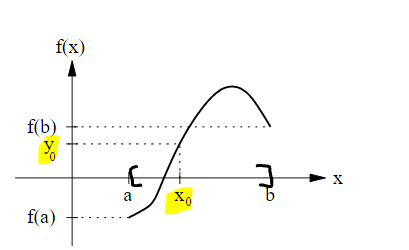
\includegraphics[width=5cm]{zws.png} \\
        \midrule
        5.7.26& \textbf{Nullstellensatz von Bolzano} \hfill \break
                Es seien $a,b \in \mathbb{R}$ mit $a < b$ gegeben und $f \in C([a,b])$ erfülle $f(a)f(b) < 0$ (Existenz einer Nullstelle /
                Einer der beiden Werte 0).
                Dann gibt es ein $x_0 \in (a,b)$ mit $f(x_0) = 0$. \\
        \midrule
        5.7.28& Es sei $K \subseteq \mathbb{R}$ \textbf{kompakt} und nicht-leer, sowie $f \in C(K)$. Dann gibt es $x_*, x^* \in K$, so dass
                $f(x_*) \leq f(x) \leq f(x^*)$ für alle $x \in K$ gilt. Insbesondere ist $f$ \textbf{beschränkt}. (Jede stetige Funktion auf 
                kompakter Menge ist beschränkt)\\

        \bottomrule
    \end{tabularx}
    \end{table}

\subsection{Stetigkeit von Funktionen mehrerer Variablen}
        \noindent
    \textbf{Definitionen}
    \begin{table}[H]  
    \begin{tabularx}{\textwidth}{X m{16cm}}
        \toprule

        5.8.1 & Es seien $V$ und $W$ normierte $\mathbb{R}$-Vektorräume, $D \subseteq V$ und $f: D \rightarrow W$ eine Funktion.
                \begin{itemize}
                    \item[a)] Wir nennen $x_0 \in D$ \textbf{Häufungspunkt} von $D$, falls es eine Folge $(a_n)$ in $D$ mit 
                                $a_n \neq x_0$ für alle $n \in \mathbb{N}$ gibt, die gegen $x_0$ konvergiert.
                    \item[b)] Sei $x_0$ ein Häufungspunkt von $D$. Dann ist $lim_{x \rightarrow x_0} f(x) = y$, falls für jede 
                                Folge $(a_n)$ in $D$, die gegen $x_0$ konvergiert und $a_n \neq x_0$ für alle $n \in \mathbb{N}$
                                erfüllt, die Folge $(f(a_n))$ gegen $y$ konvergiert.
                \end{itemize} \\
        \midrule
        5.3.8 & Es seien $V,W$ zwei normierte $\mathbb{R}$-Vektorräumen, $D \subseteq V$ und $x_0 \in D$. Eine Funktion $f: D\rightarrow W$
                heißt \textbf{stetig} in $x_0$, wenn für jede Folge $(a_n)$ in $D$, die gegen $x_0$ konvergiert, auch die Folge
                $(f(a_n))$ konvergiert und $lim_{n \rightarrow \infty} f(a_n) = f(x_0)$ gilt. \hfill \break
                Weiter heißt \textbf{f stetig auf D}, wenn $f$ in jedem Punkt $x_0 \in D$ stetig ist. \hfill \break
                Au\ss erdem setzen wir wieder $C(D;W) := \{f: D\rightarrow W: f$ stetig auf $D$\}. \\

        \bottomrule

    \end{tabularx}
    \end{table}

    \noindent 
    \textbf{Sätze}
    \begin{table}[H]
    \begin{tabularx}{\textwidth}{X m{16cm}}
        \toprule

        5.8.4 & Es sei $D \subseteq \mathbb{R^d}$ und $x_0 \in D$. Dann ist $f: D \rightarrow \mathbb{R^p}$ genau dann in $x_0$
                \textbf{stetig}, wenn alle Koordinatenfunktionen $f_1, f_2, \dots, f_p : D \rightarrow \mathbb{R}$ in $x_0$ stetig sind. \\
        \midrule
        5.8.5 &  Es seien $D \subseteq \mathbb{R^d}$, $x_0 \in D$ und $f,g : D \rightarrow \mathbb{R}$ stetig in $x_0$, sowie
                $h : f(D) \rightarrow \mathbb{R}$ stetig in $f(x_0)$. Dann sind auch $f+g$, $fg$ und $h \circ f$ als Funktionen
                von $D$ nach $\mathbb{R}$ stetig in $x_0$. \hfill \break
                Ist au\ss erdem $x_0 \in D^* := \{x \in D: g(x) \neq 0\}$, so ist auch $\frac{f}{g}:D^* \rightarrow \mathbb{R}$ stetig in $x_0$. \\
        \midrule
        5.8.8 & Es sei $K \subseteq \mathbb{R^d}$ \textbf{kompakt} und nicht-leer, sowie $f \in C(K)$. Dann gibt es $x_*, x^* \in K$, so dass \hfill \break
                \centerline{$f(x_*) \leq f(x) \leq f(x^*)$ für alle $x \in K$}
                gilt. Insbesondere ist $f$ \textbf{beschränkt}. \\
        \bottomrule
    \end{tabularx}
    \end{table}

    \noindent
    \textbf{Bemerkungen}
    \begin{table}[H]
    \begin{tabularx}{\textwidth}{X m{16cm}}
        \toprule

        5.8.2 & Hier keine links- und rechtsseitiger Grenzwerte, da es Unmengen an Richtungen gibt \\

        \bottomrule
    \end{tabularx}
    \end{table}

    \noindent
    \textbf{Beispiele}
    \begin{table}[h]
    \begin{tabularx}{\textwidth}{X m{16cm}}
        \toprule

        & \\

        \bottomrule
    \end{tabularx}
    \end{table}
\end{document}